\documentclass[journal = jacsat, manuscript = suppinfo]{achemso}

\usepackage{mhchem}
\usepackage{graphicx}
\usepackage{mwe}

\makeatletter
\def\acs@author@fnsymbol#1{}
\makeatother

\SectionNumbersOn

\newcommand{\barf}{\ce{BAr^F_4^-}}
\newcommand{\nabarf}{\ce{NaBAr^F_4}}
\newcommand{\nabf}{\ce{NaBF4}}
\newcommand{\brarf}{\ce{BrC6H3-3,5-(CF3)2}}
\newcommand{\fnmr}{$^{19}$F NMR}
\newcommand{\hnmr}{$^{1}$H NMR}

\title{Synthesis, Purification, and Analysis of the Weakly-Coordinating Anion \barf}

\author{David Qiu}
\affiliation{Department of Chemistry, University of Illinois at Urbana-Champaign, 505 S Matthews Avenue, Urbana, IL, 61801}
\email{davidlq2@illinois.edu}

\begin{document}

\tableofcontents

\section{General Considerations}

A 60 MHz Nanalysis NMReady-60PRO tabletop NMR instrument coupled with a STC-1000
digital temperature controller was used to record all \fnmr\ and \hnmr\
spectra. NMR spectra were taken in DMSO-d6 sourced from Cambridge Isotope
Laboratories, Inc. Activated carbon charcoal and benzene was sourced from EMD
Millipore.  Sodium sulfate was sourced from Alfa Aesar. Mg and \nabf\ were
sourced from Sigma-Aldrich. \brarf\ was sourced from Oakwood Chemicals.
1,2-dibromoethane and diethyl ether were sourced from Fisher Chemicals.
Air and moisture-free experimental conditions were achieved with a Schlenk line
following standard procedure unless specified otherwise.

\section{Materials and Methods}

\subsection{Synthesis of \nabarf}

To a 500 mL three-necked round-bottom flask was added 1.17 g (48.1 mmol) of
magnesium turnings, 0.813 g (7.40 mmol) \nabf, and a stir bar. A reflux
condenser, an addition funnel, and a rubber septum secured with copper wire were
fit on each neck.  The appartus was attached to the Schlenk line, and
was vacuumed and refilled with nitrogen three times. Using an airtight syringe,
75 mL of diethyl ether was added to the flask, followed by 0.57 mL (6.7
mmol) of 1,2-dibromoethane added similarly. The mixture was then heated on
a heating mantle attached to a 40 V Variac until the solution began to
bubble softly and turn a cloudy gray, signaling the initiation of the
magnesium turnings.

Upon initiation, the heating mantle was removed from contact with the system,
and the solution was allowed to continue stirring until the reflux ceased. While
the flask cooled, 7.15 mL (41.5 mmol) of \brarf\ was mixed with 50 mL of diethyl
ether and injected into the separate, closed addition funnel.  While the
solution inside the flask was warm, but no longer refluxing, the addition
funnel's stopcock was turned slightly to allow the dropwise addition of the
\brarf\ solution over the course of 30 minutes. The flask solution gradually
darkened into a caramel brown, indicative of successful \barf\ synthesis.

Upon complete addition of the \brarf\ solution, the reaction mixture was then
refluxed again for 30 minutes on a heating mantle attached to a 40 V Variac.
Afterwards, the solution was allowed to cool to room temperature, and the
experimental appartus was disassembled quickly to minimize exposure of the
\nabarf\ solution to ambient conditions. The round-bottom flask containing the
newly-synthesized \nabarf\ solution was sealed with glass stoppers, and stored at
room temperature for a week.

\subsection{Purification of \nabarf}

The \nabarf\ solution was transferred into a 1 L separatory funnel, and washed
with 50 mL of diethyl ether and 100 mL of brine, followed by a second washing
with 100 mL of DI water. The organic \nabarf\ solution was collected into a 500
mL Erlenmeyer flask, was dried with 27 g of sodium sulfate, and was de-colored
with 2 g of activated carbon charcoal. The solution was mixed vigorously for
five minutes, and was filtered through a Buchner funnel into a 500 mL three-necked
round-bottom flask. The side necks were sealed with rubber septa and copper
wire, and the \nabarf\ solution was dried with a rotary evaporator to yield a
thick, dark-brown oil.

A standard Dean-Stark apparatus was then assembled with the \nabarf\ flask, and
was connected to the Schlenk line under an inert nitrogen atmosphere. 100 mL of
benzene was injected into the flask, and the solution was heated until 75 mL of
organic and aqueous solvent had been removed. The \nabarf\ solution was dried again
using a rotary evaporator, unfortunately yielding a thick, dark-brown \nabarf\
slurry which failed to dry under 10 minutes of vacuum on the Schlenk line.

The purified \nabarf\ sample was then weighed, and a small sample was saved for
NMR analysis. The measured yield of this reaction was 6.825 g (104\% yield),
which is likely inaccurate due to the residual solvent unable to be removed from
the system.

\section{Analysis of \nabarf}

Unfortunately, the NMR instrument had a severe software malfunction near the end
of the last experimental period, and NMR data was unable to be obtained for the
\nabarf\ sample. Sample \hnmr\ and \fnmr\ spectra of \nabarf\ in deuterated
acetone collected via a 400 MHz Bruker NMR instrument were provided by the TAs
and analyzed.

\begin{figure}
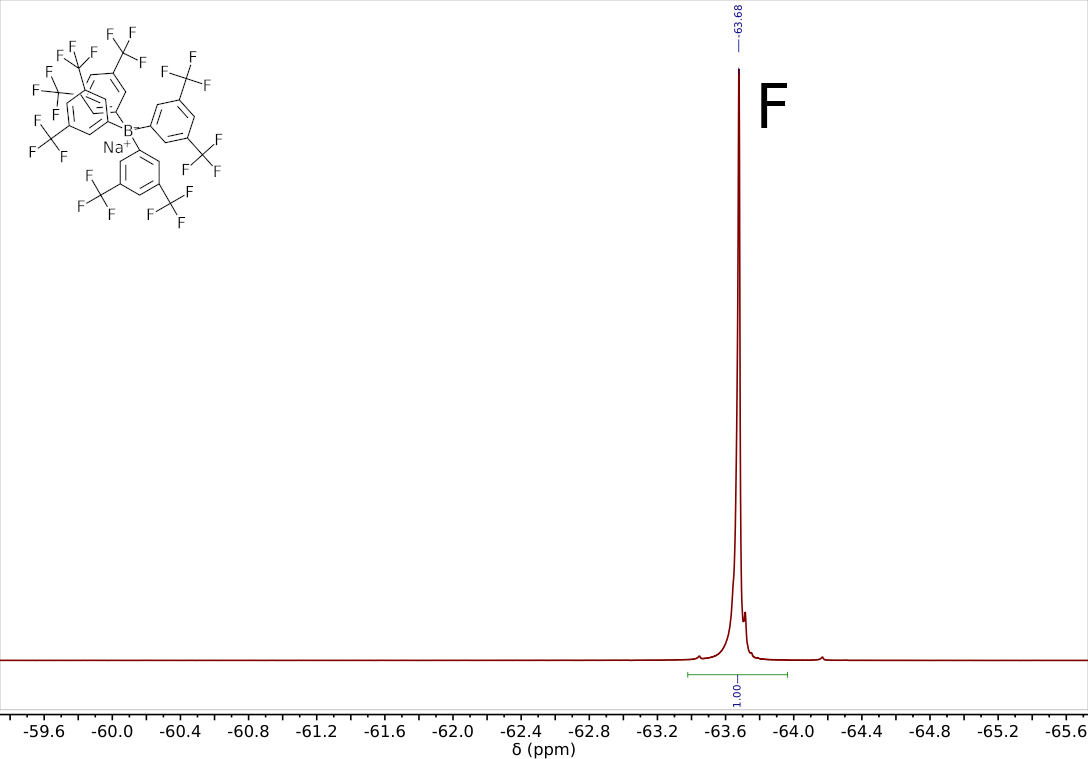
\includegraphics[width=\textwidth]{figures/fnmr.png}
\caption{Provided \fnmr spectra of \nabarf .}
\end{figure}

\begin{figure}
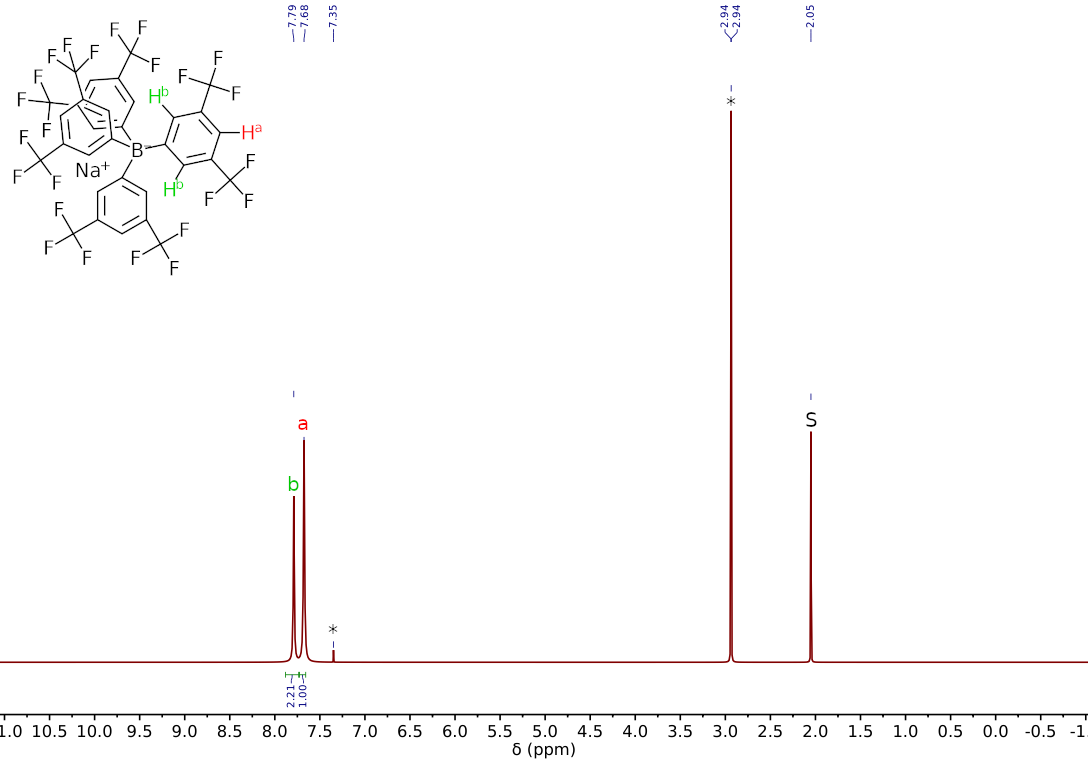
\includegraphics[width=\textwidth]{figures/hnmr.png}
\caption{Provided \hnmr spectra of \nabarf . ``S" denotes residual
non-deuterated acetone present in the solvent, and ``*" denotes an unidentified
impurity.}
\end{figure}

The NMR interpretation is as follows. \fnmr: $\delta$ 63.68 (s, 24 F). \hnmr:
$\delta$ 7.68 (d, 8 H), 7.68 (d, 4 H). The NMR spectra and their interpretation
are in excellent agreement with those of existing literature \cite{barfnmr}.

\bibliography{lab_2_si.bib}

\end{document}
